\documentclass{article}
\usepackage{amsmath}
\usepackage{float}
\usepackage{hyperref}
\usepackage{geometry}
 \geometry{
 a4paper,
 total={170mm,257mm},
 left=20mm,
 top=20mm,
 }

\usepackage{graphicx}
\graphicspath{ {./images/} }


\title{PH456 Lab 1 : Random Numbers} % Sets article title
\author{Sourabh Choudhary} % Sets authors name
\date{\today} % Sets date for date compiled

% The preamble ends with the command \begin{document}
\begin{document} % All begin commands must be paired with an end command somewhere
    
\maketitle % creates title using information in preamble (title, author, date)

The code is available on github via this \href{https://github.com/sourabh-ch/ph456-computational}{link}. 
All code is in lab-1 folder code for \textbf{Task 1} is in lab-1.ipynb and for \textbf{Task 2 to 4} is in lab-1-task2-4.py.

\section{Generating random numbers from different initial seeds} % creates a section
    
Two sets of random numbers were generated, first using python built-in module \textbf{random} 
and installed library \textbf{numpy}.

\begin{figure}[H]\label{fig:RNGs2D}
    \centering
    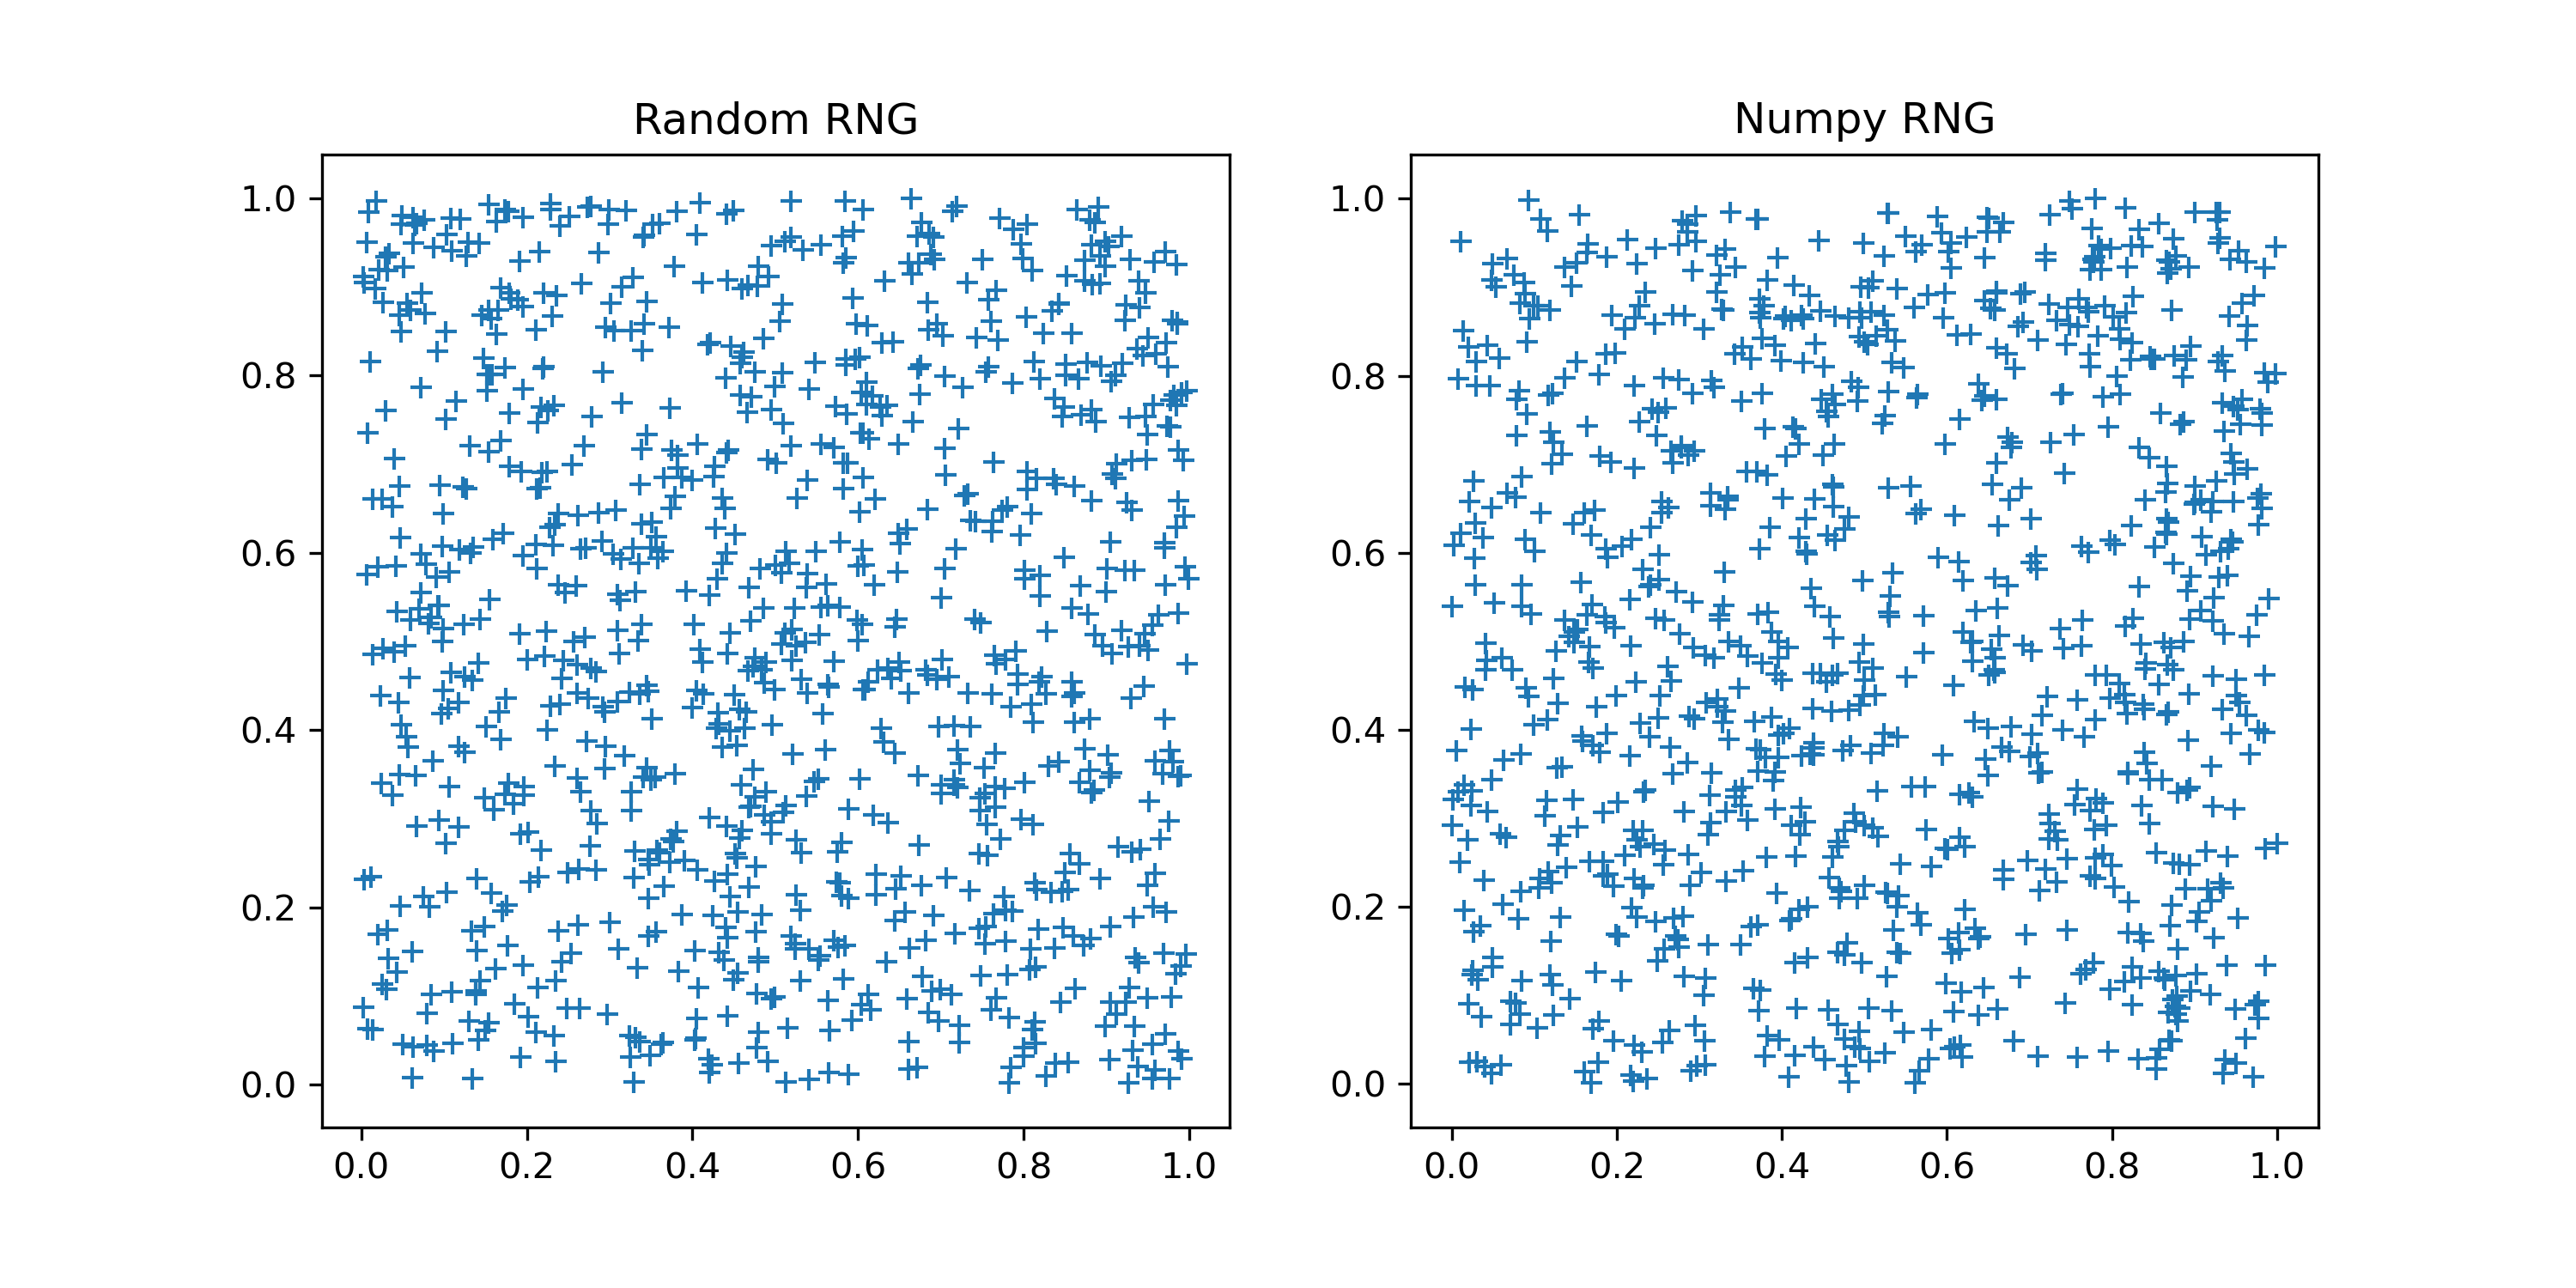
\includegraphics[scale = 0.5]{task1.png}
    \caption[Random Numbers]{These figures show 1000 random numbers plotted in 2D. The figure
    on the left shows the random numbers generated using the python built module \textbf{random}. 
    The figure on the right shows the numbers generated using the library \textbf{numpy}.}
\end{figure}

\subsection{Testing for unifomity using $ \chi^2 $ test:}

The uniformity for both random number generators (RGNs) is visualised in Figure \ref{fig:RNGs2D} used 
and was tested using the $ \chi^2 $ test. Following equations show the results for the python 
built-in module \textbf{random} and for the numbers generated using the library \textbf{numpy} 
respectively. 

\begin{equation}
    \chi^2_1 = 83, p=0.88 
\end{equation}

\begin{equation}
    \chi^2_2 = 94, p=0.62
\end{equation}


To do the $ \chi^2 $ test the \textbf{frequencies} function was written to generate the frequency 
distribution for the random number using given array of numbers and number of bins. 

Test was done with random numbers N = 1000, Bins = 100. From the results we can see in both cases 
$ \chi^2 < 100 $. This shows that the generated random numbers are uniform 
and pass this test. The p values show the probability of obtaining $ \chi^2 \geq $  
current value and still pass the test. 

\subsection{Auto-correlation :}
Using the statsmodels library the autocorrelation function for 100 Random numbers was plotted
as shown below:

    \begin{figure}
        \begin{minipage}[c]{0.5\textwidth}
        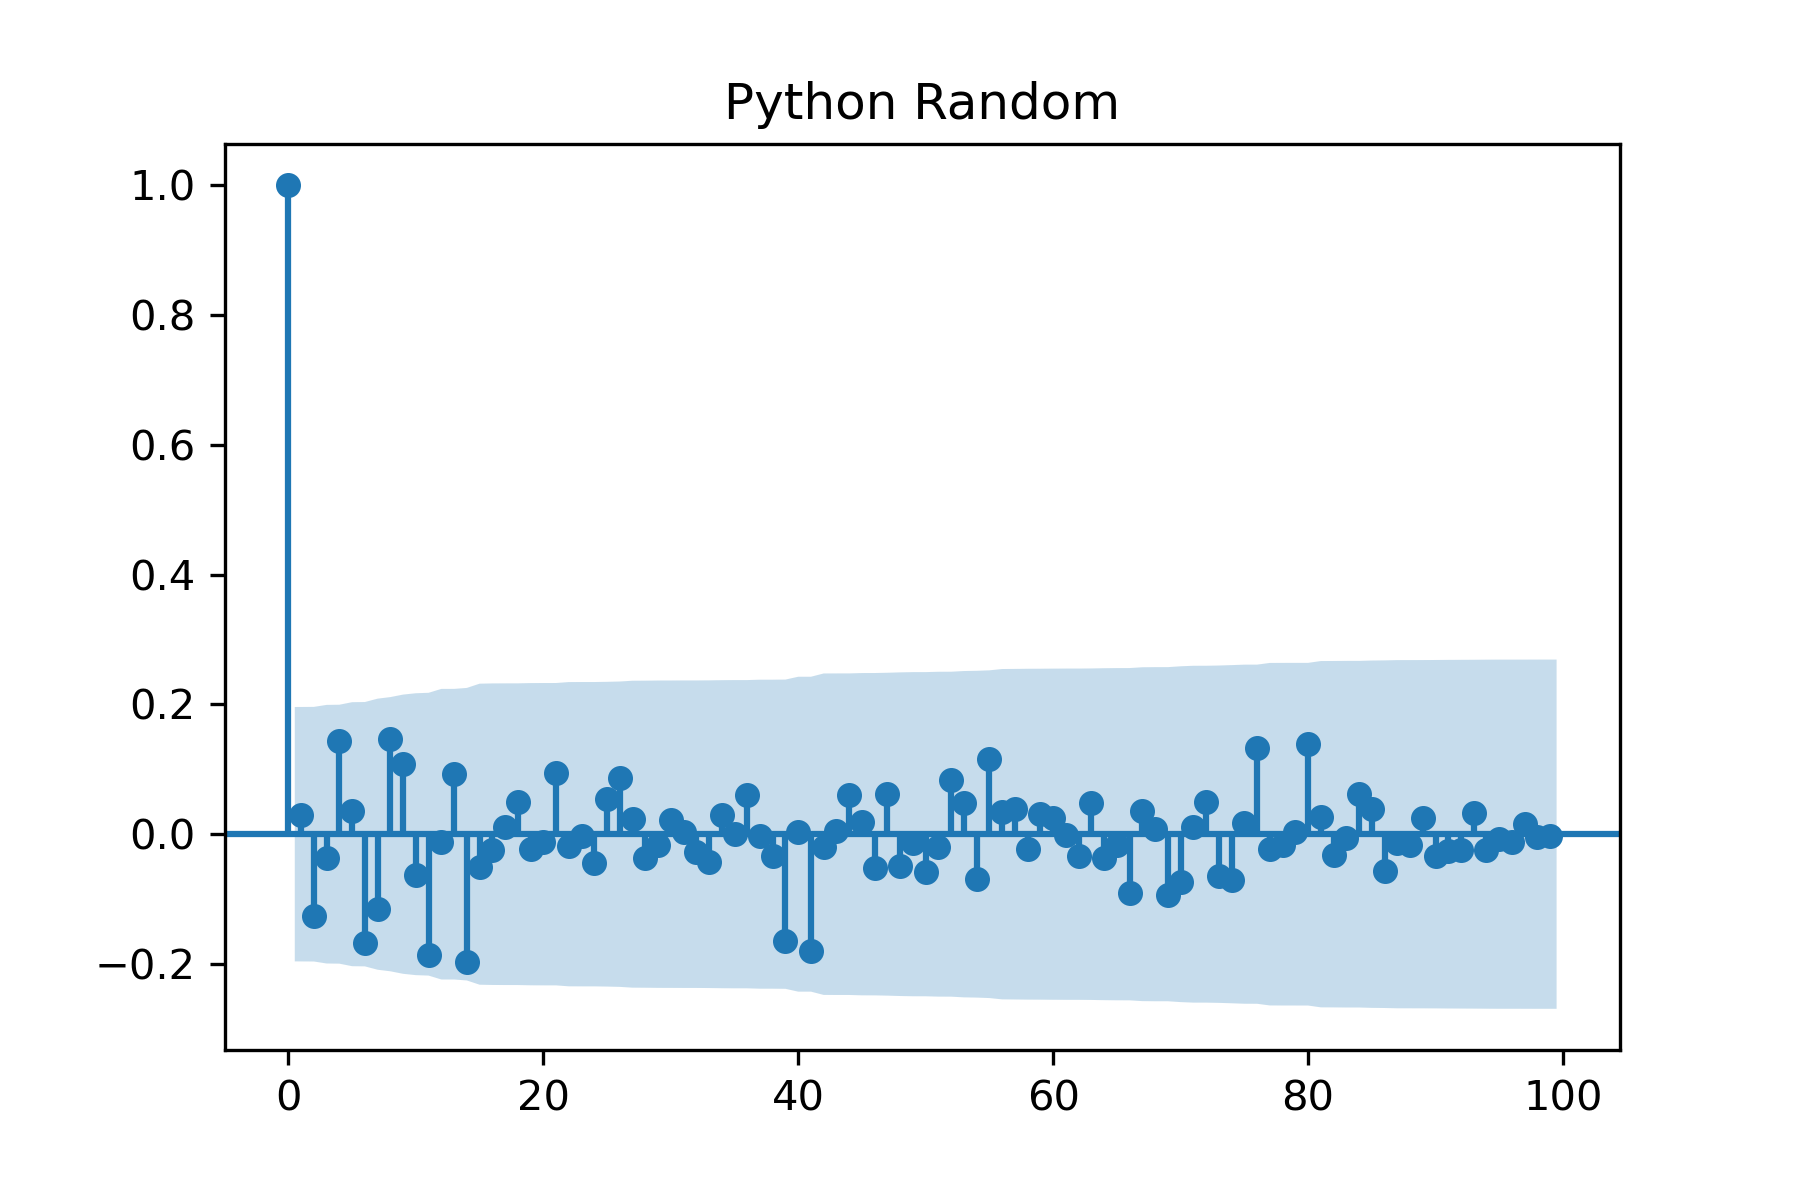
\includegraphics[width=\textwidth]{task1a1.png}
        \end{minipage}\hfill
        \begin{minipage}[c]{0.5\textwidth}
        \caption{
            Figure on left shows the auto-correlation for 100 Random Numbers generated using python
            built-in module \textbf{random}.
            The scale works measures the correlation on a scale 
            between 1 and -1. With 1 indicating a 100 \% positive correlation and -1 indicating a negative 
            correlation. The shaded portion represents the confidence interval determined using 
            Bartlett's formula, plotted here with a 95 \% confidence interval. Points in the shaded 
            region show that there is no significant correlation.
        } \label{fig:2a}
        \end{minipage}
    \end{figure}

    \begin{figure}
        \begin{minipage}[c]{0.5\textwidth}
        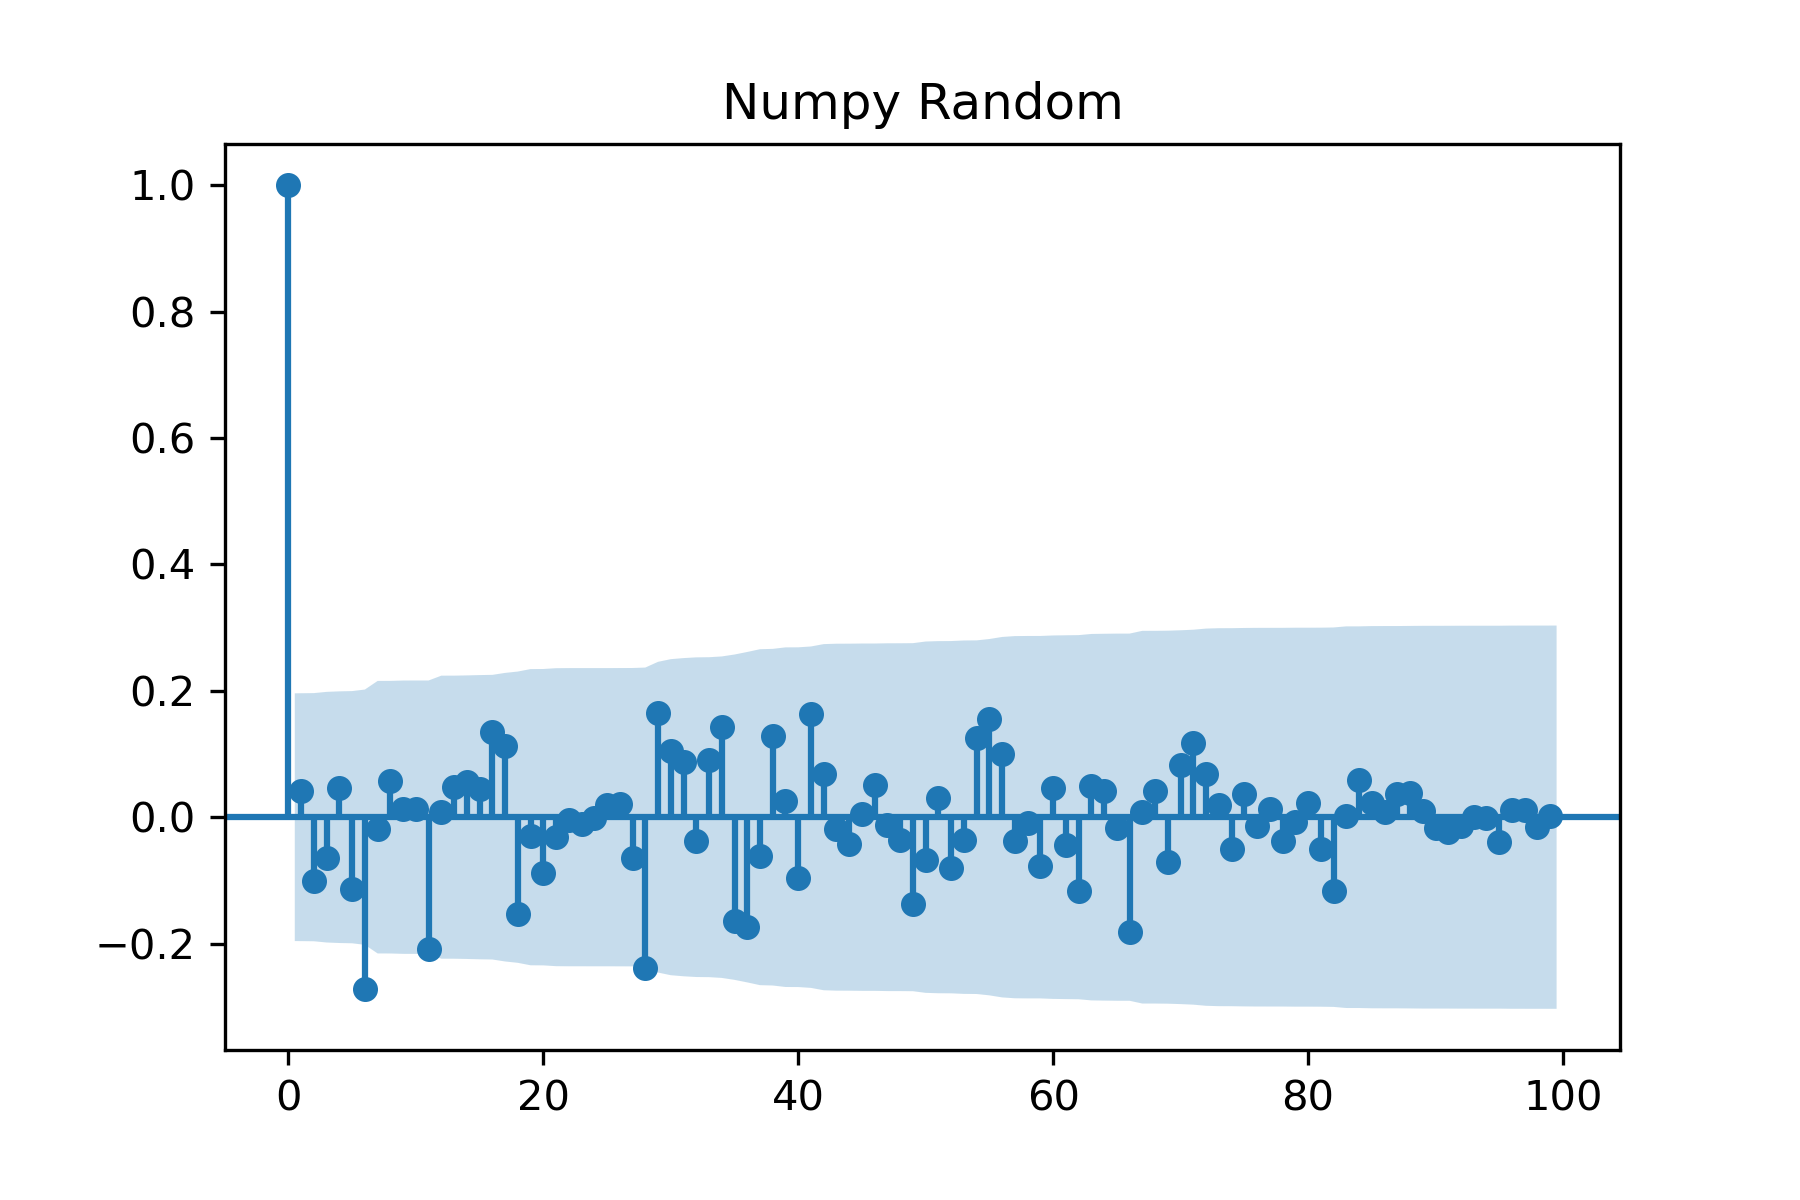
\includegraphics[width=\textwidth]{task1a2.png}
        \end{minipage}\hfill
        \begin{minipage}[c]{0.5\textwidth}
        \caption{
            Figure on left shows the auto-correlation for 100 Random Numbers generated using
            \textbf{numpy} library. With a similar interpretaion as in the previous figure, this
            too shows that there is no significant correlation between the numbers generated.
        } \label{fig:2b}
        \end{minipage}
    \end{figure}

\section{Simulating a Partitioned Box:}

Running the \textbf{lab-1-task2-4.py} will start the animation of the particle simulator. The 
simulator was built using the code found on 
\href{https://scipython.com/blog/the-maxwellboltzmann-distribution-in-two-dimensions/}{this website}.

\noindent
Comments have been added with guidlines to the code to switch between the different RNGs 
for inital conditions of the simulations.

\section{Partitioned box simulations:}

\subsection{Using built-in module random for inital conditions:}

\begin{figure}[H]
    \begin{minipage}[c]{0.5\textwidth}
    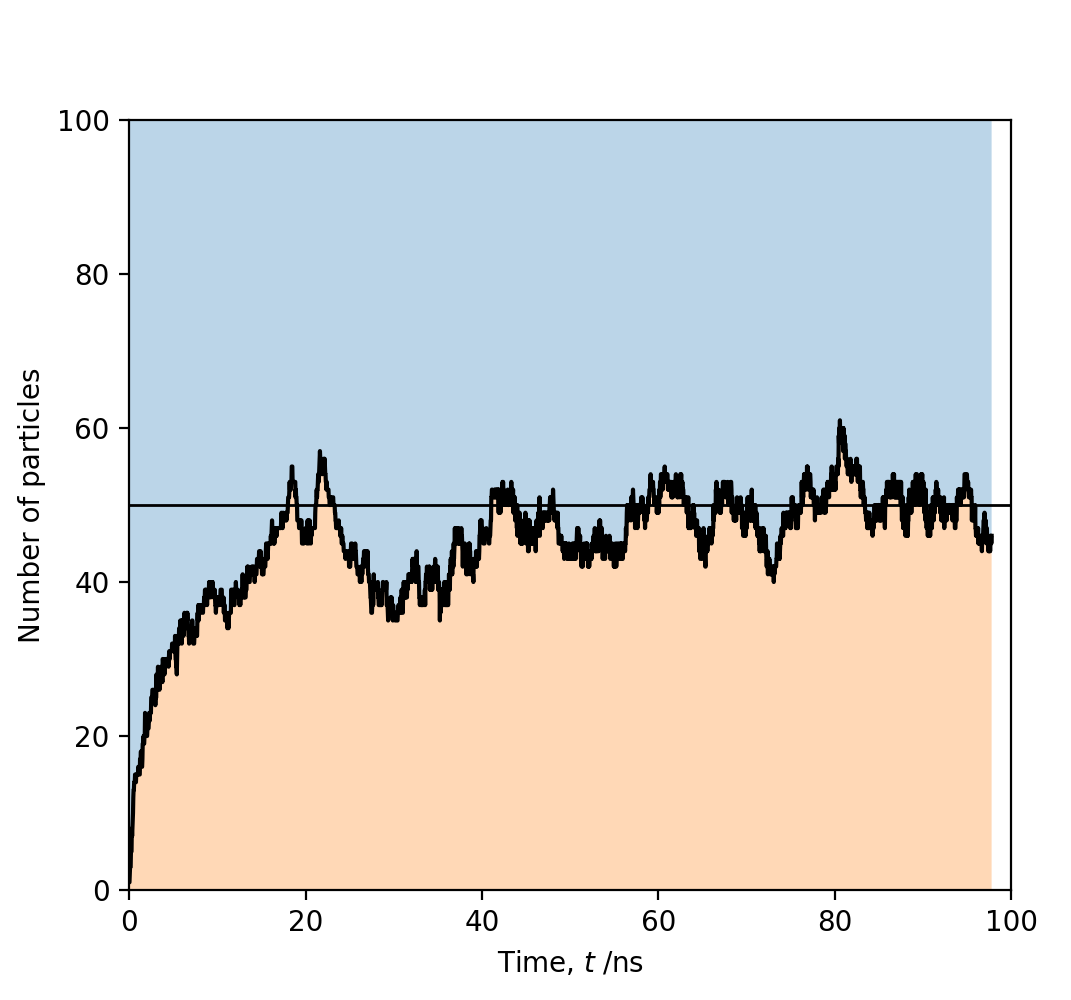
\includegraphics[width=\textwidth]{Figure_3a.png}
    \end{minipage}\hfill
    \begin{minipage}[c]{0.5\textwidth}
    \caption{
        Figure on left shows simulation for 100 particles with inital positions generated using 
        \textbf{random} module, the velocities and orientations were also generated using the same.
        Particles are \textit{on average} equally distributed in the two sides as expected. 
    } \label{fig:3a}
    \end{minipage}
\end{figure}


\subsection{Using numpy random numbers for inital conditions:}

\begin{figure}[H]
    \begin{minipage}[c]{0.5\textwidth}
    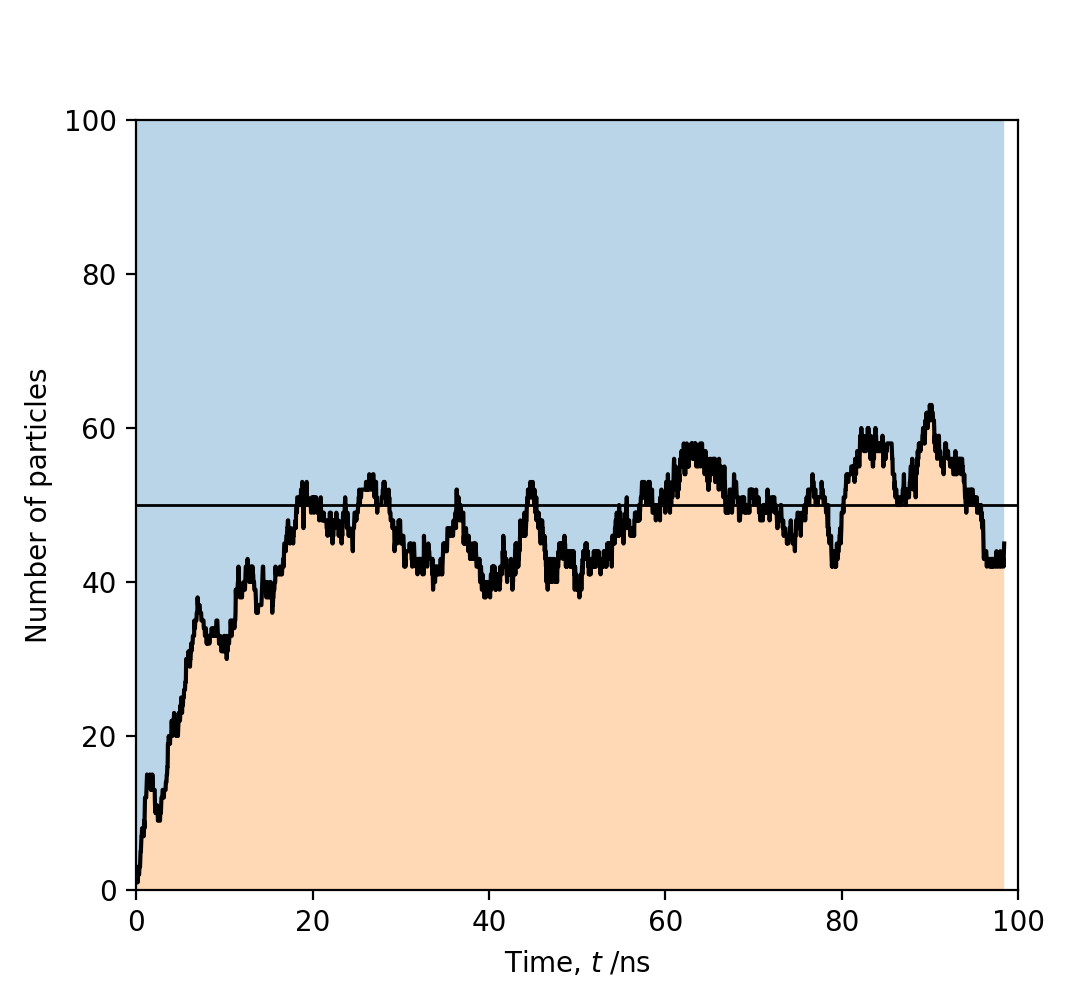
\includegraphics[width=\textwidth]{Figure_3b.png}
    \end{minipage}\hfill
    \begin{minipage}[c]{0.5\textwidth}
    \caption{
        Figure on left shows simulation for 100 particles with inital positions generated using 
        \textbf{numpy} library, the velocities and orientations were also generated using the same.
        Results are similar as seen before.
    } \label{fig:3b}
    \end{minipage}
\end{figure}

\section{75:25 Probabilty for the partitioned box :}

\begin{figure}[H]
    \begin{minipage}[c]{0.5\textwidth}
    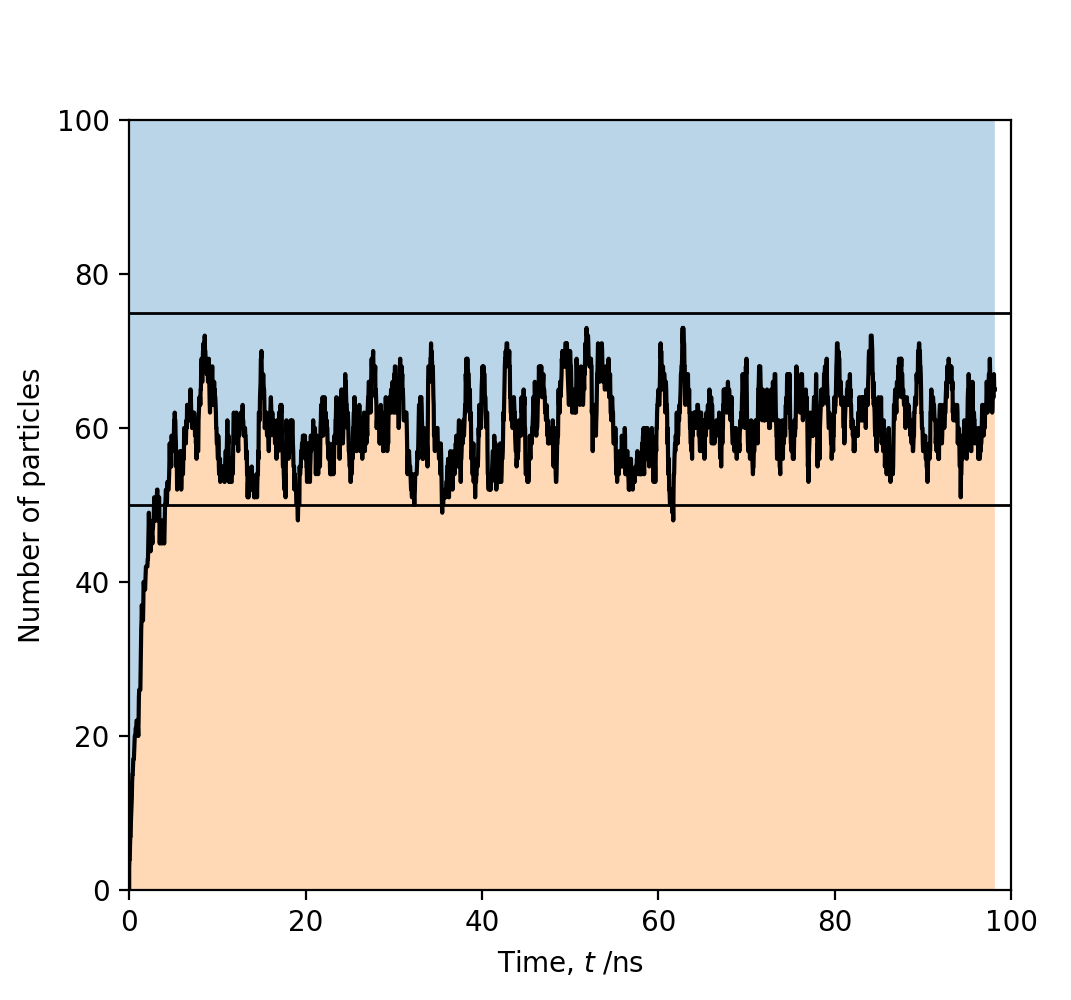
\includegraphics[width=\textwidth]{Figure_4.png}
    \end{minipage}\hfill
    \begin{minipage}[c]{0.5\textwidth}
    \caption{
        The intention of this simulation was to have 75 \% of the particles on one side of the box.
        Attempted to achieve this by manipulating the reaction that particle has on hitting the 
        middle wall, but it did not work as intended.
    } \label{fig:4}
    \end{minipage}
\end{figure}

\section{Link}

\href{https://github.com/sourabh-ch/ph456-computational}{github repository}

\end{document} % This is the end of the document